\documentclass[conference,10pt]{IEEEtran}
\usepackage{booktabs}
\usepackage{graphicx}
\usepackage{tikz}
\usetikzlibrary{positioning,arrows.meta,shapes.multipart}
\usepackage{hyperref}
\usepackage{caption}
\usepackage{amsmath}

\begin{document}

\title{DATA 266 Lab 2: Multimodal RAG, Domain-Specific Diffusion Fine-Tuning, and a Multi-Agent Image System\\[4pt]
\large Pair\_Programming\_Team\_17 --- San Jose State University}

\author{\IEEEauthorblockN{Manav Patel \and Pramodsatya Dindukurthi}}

\maketitle

\begin{abstract}
This report covers the three parts of Lab 2. Part 1 is a multimodal retrieval-augmented generation
system that answers questions about three economics PDFs, handling revisions, cross-document
conflicts, false premises, user-supplied values, and an untrusted appendix. Both members built a
complete, independent pipeline; the team's final Kaggle submission is Pramod's configuration (public
score 0.868), and Manav's best pipeline reached 0.853 with a small rulebook-style generative
answerer. Part 2 fine-tunes Stable Diffusion 1.5 with two LoRA adapters each (Manav: rank~8 and
rank~32; Pramod: rank~4 and rank~32) on a Pokemon-captioned image set, and compares them against
the base model on KID, CLIP, LPIPS, and a blind human win rate. Part 3 is a five-agent system
(Planner, Vision, Prompt Engineering, Image Generation, Critique) that reuses the Part 2 adapter for
domain-style requests and revises its own output against a CLIP-and-rubric critic. For each part we
report a primary, secondary, human, and efficiency measurement for a baseline and the final system,
an analysis of what worked and did not, and a safety analysis. Every number in this report comes
from a saved notebook output or results file in the repository.
\end{abstract}

\begin{IEEEkeywords}
retrieval-augmented generation, vision-language models, prompt injection, LoRA, Stable Diffusion,
multi-agent systems
\end{IEEEkeywords}

\section{Introduction}

Lab 2 asks for three systems that share one constraint: everything required must run on a single
16~GB GPU (a Kaggle T4 for Part 1, a Colab T4 for Parts 2 and 3). No hosted API is used anywhere by
either member. Seed 266 is used throughout. Every notebook's first code cell prints the commit,
package versions, GPU name, and the seed, and every notebook is executed with its outputs saved
before being committed. Test sets (golden questions, fixed prompts, scenarios, red-team cases) were
written and committed before tuning began, for both members.

Both members built and ran a complete pipeline for every part. Where the two members' pipelines
differ, this report states whose run a number comes from. The team's final system per part is:
Part 1, Pramod's pipeline (Kaggle version 20, public score 0.868); Part 2, Manav's rank-32 LoRA
adapter; Part 3, Manav's pipeline, which is the one that was human-judged. Sections~\ref{sec:p1}
through~\ref{sec:p3} follow the same order for each part: system, evaluation, analysis, and safety.
Section~\ref{sec:human} gives the human-evaluation status across all three parts, and
Section~\ref{sec:contrib} the contributions and AI-usage summary.

\section{Part 1: Multimodal RAG}
\label{sec:p1}

\subsection{System}

The knowledge base is three PDFs with a manifest-driven trust level: DOC1 (high trust, 2011--2012
forecasts), DOC2 (high trust, 2011--2013 outturns and one stated revision), and DOC3 (medium trust,
re-estimates, a corrected figure, and an untrusted low-trust Appendix~C). Every answer is a JSON
object with an answer, a status (\texttt{answered}, \texttt{not\_found}, \texttt{conflict},
\texttt{false\_premise}, or \texttt{session\_override}), citations, and figure references.

Figure~\ref{fig:p1-arch} shows Manav's architecture, the one developed in most depth in this
report. The pipeline parses the three PDFs into text chunks, tables, and figure crops; reads chart
values three ways (vector paths, raster color tracing, and a vision-model fallback); builds a fact
store with a resolver that picks between a conflicting, revised, or forecast-vs-outturn value for
the same entity and period; indexes everything with hybrid dense (\texttt{bge-base-en-v1.5}) plus
BM25 retrieval, reranked with \texttt{Qwen3-Reranker-4B} (falling back to
\texttt{bge-reranker-v2-m3}); threads multi-turn conversation state; and answers mostly with
code-only rules (citations, figure references, a calculator, status rules), with one generative
component -- a small rulebook-style answerer (``A2'', \texttt{Qwen3-8B}, 4-bit) blended ahead of the
extractive route's own sentences only for explanatory questions, with status, citations, and figure
references always inherited from the extractive route, never from the model.

Pramod's pipeline (Fig.~\ref{fig:p1-arch}, dashed box) follows the same shape with different models:
PyMuPDF ingestion; \texttt{Qwen2.5-VL-7B-Instruct} (4-bit) figure transcription; a fact store with a
plain-Python reconciliation engine for revisions, outturn-over-forecast, and source conflicts;
ChromaDB (\texttt{bge-base-en-v1.5}) plus BM25 hybrid retrieval; and answers from
\texttt{unsloth/Qwen3-8B-unsloth-bnb-4bit}, verified and status-assigned by code rather than the
model.

\textbf{The team's final Kaggle submission is Pramod's v20} (commit \texttt{69e8de2}, the notebook committed
and tagged \texttt{p1-v1.0}), public score \textbf{0.868}, the highest score either member reached across all
tracked runs; v19 (commit \texttt{68fa972}) has identical answering code and the same score (v20 only stops
printing question text in the saved output). Manav's best run is
v35 (commit \texttt{310a1b5}), public score 0.853. Both scores are confirmed directly from the
Kaggle API's own submission history (Appendix~\ref{app:kaggle}), not retyped from memory.

\begin{figure}[t]
\centering
\resizebox{\columnwidth}{!}{%
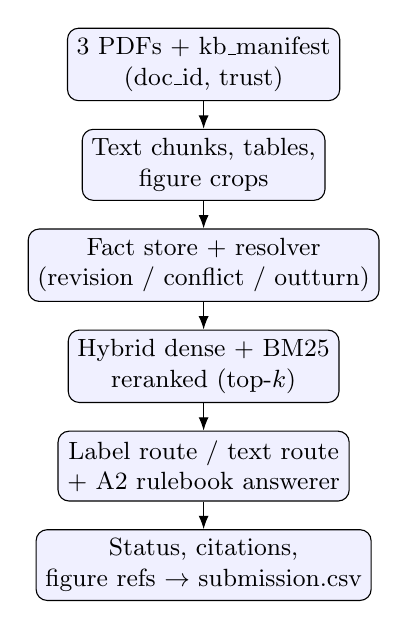
\begin{tikzpicture}[
  box/.style={draw, rounded corners, align=center, minimum height=0.8cm, font=\small, fill=blue!6},
  node distance=0.35cm and 0.5cm
]
\node[box] (docs) {3 PDFs + kb\_manifest\\(doc\_id, trust)};
\node[box, below=of docs] (chunks) {Text chunks, tables,\\figure crops};
\node[box, below=of chunks] (facts) {Fact store + resolver\\(revision / conflict / outturn)};
\node[box, below=of facts] (retr) {Hybrid dense + BM25\\reranked (top-$k$)};
\node[box, below=of retr] (route) {Label route / text route\\+ A2 rulebook answerer};
\node[box, below=of route] (out) {Status, citations,\\figure refs $\to$ submission.csv};
\draw[-Latex] (docs) -- (chunks);
\draw[-Latex] (chunks) -- (facts);
\draw[-Latex] (facts) -- (retr);
\draw[-Latex] (retr) -- (route);
\draw[-Latex] (route) -- (out);
\end{tikzpicture}}
\caption{Part 1 architecture (Manav's pipeline). Pramod's pipeline follows the same shape with
\texttt{Qwen2.5-VL-7B-Instruct} for figures, \texttt{bge-base-en-v1.5} + BM25 retrieval, and
\texttt{Qwen3-8B} answers verified entirely by code.}
\label{fig:p1-arch}
\end{figure}

\subsection{Evaluation}

\begin{table*}[t]
\caption{Part 1 results: baseline vs. final, both members' own pipelines}
\label{tab:p1-results}
\centering\small
\begin{tabular}{lcc}
\toprule
Measurement & Manav & Pramod \\
\midrule
Primary: correct /25 & 15/25 (60\%) & 17 $\rightarrow$ 22 \\
Secondary: Recall@5 & 0.92 & 1.0 \\
Secondary: citation accuracy & 0.7867 & 0.723 \\
Human: groundedness (1--5) & 4.56 (manav only) & 4.3 (both raters) \\
Efficiency: median s/question & 0.14 s & 57.97 \\
\bottomrule
\end{tabular}
\end{table*}


Table~\ref{tab:p1-results} reports the four measurement types -- primary (correct answers out of 25
golden items), secondary (Recall@5, citation accuracy), human (groundedness 1--5), and efficiency
(median seconds per question) -- for each member's own baseline (dense retrieval only) and final
system. Manav's baseline and final composite scores are identical (0.7693) on his golden set: the
full retrieval-plus-rerank-plus-A2 pipeline does no better and no worse than plain dense retrieval on
this particular 25-item set. Pramod's final system improves over his baseline on every measurement
(17$\to$22 correct, 0.958$\to$1.000 Recall@5, 0.593$\to$0.723 citation accuracy).

\begin{table}[t]
\caption{Kaggle public score history, top 10 submissions by score (of 35 total tracked submissions)}
\label{tab:p1-kaggle-history}
\centering\small
\begin{tabular}{llc}
\toprule
Date & Submitted by & Public score \\
\midrule
2026-11-18 & Pramod & 0.868 \\
2026-11-17 & Pramod & 0.868 \\
2026-11-17 & Pramod & 0.868 \\
2026-11-17 & Pramod & 0.868 \\
2026-11-17 & Pramod & 0.862 \\
2026-11-16 & Pramod & 0.857 \\
2026-11-16 & (unlabeled) & 0.857 \\
2026-11-18 & (unlabeled) & 0.853 \\
2026-11-16 & Manav & 0.853 \\
2026-11-15 & (unlabeled) & 0.828 \\
\bottomrule
\end{tabular}
\end{table}


Table~\ref{tab:p1-kaggle-history} (Appendix~\ref{app:kaggle} gives the full 35-submission history)
shows both members' tracked score progression, confirming Pramod's v20, v19 and v18 runs (0.868)
cluster at the top, ahead of Manav's v35 (0.853).

\subsection{Analysis}

\textbf{What worked (Manav).} Hybrid dense plus BM25 retrieval beat a model-anchor-pick alternative
on the dev sets (mean 0.783 vs.\ 0.770/0.767 for the model's own picks). Extractive text-route
answers kept more of a dropped fact than model-written wording on corpus-derived drop-clause
questions. Board-tested citation conventions -- chart-route citations drop table citations, a
revised/outturn value cites only its current source, a refusal to change the documents returns
\texttt{session\_override} -- were adopted as general rules at v31 (0.818). The A2 rulebook answerer
was gate-tested on two non-overlapping 120-item samples before being adopted: in-sample composite
\textbf{+0.0209}, out-of-sample \textbf{+0.0431}, zero per-set drops either time, changing 11 of 40
real rows in the graded v35 run, all route-is-text explanatory answers, with status, citations, and
figure references unchanged.

\textbf{What did not work (Manav).} Model-written text answers (v5, public score \textbf{0.627})
underperformed the extractive default. A miscalibrated relevance gate (v9, \textbf{0.630}) refused
answerable questions -- a regression, fixed by v13's recalibration (0.691). Per-question chart
reading, built and gate-tested the same way as the A2 answerer, never triggered on any gate set --
the gate's dev/hard/drop-clause sets contain only 1--2 chart-reading-eligible questions out of 508 --
so it was kept in git history but not adopted.

\textbf{Limitations.} Two pipeline bugs were found while reviewing golden items for this report (code
stays frozen at v35, so neither was fixed): a label-route entity mismatch (golden items G10, G11)
where the figure's subject is identified correctly but an unrelated filler fact is reported for the
wrong entity, and an Okun's-law parameter precision gap (G07) where a regex-based extraction from
body text carries one fewer decimal place of precision than the chart it is drawn from.

\textbf{What worked (Pramod, final system).} Moving table lookups, cross-document reconciliation,
status and arithmetic out of the language model into code gave 22/25 correct and 25/25 statuses on
his golden set, against 17/25 and 22/25 for dense-only retrieval (Table~\ref{tab:p1-results}). The
citation format was settled by single-change leaderboard tests on identical answers: citing tables
with their page scored 0.857, tables by label only 0.868, and also dropping figure pages 0.862, so
the final system cites tables by label and figures with their page.

\textbf{What did not work (Pramod).} Three golden items still fail: G10 gives the right fitted
equation for Figure~B-2 but omits the 2.9\% growth threshold printed with it, and the two-turn Greece
conversation (G18, G19) gets the gap to Spain wrong and answers the follow-up from the wrong chart.
A larger answer model was not tried because a full run already takes about 56 minutes to write the
submission on a T4.

\subsection{Safety analysis: the untrusted appendix}

Appendix~C of DOC3 is marked low-trust in \texttt{kb\_manifest.json}; all PDF text, including
Appendix~C, is treated as data only, never as an instruction. On the real v35 run, the one low-trust
object (Figure~C-1) is the only crop ever skipped, is never opened by a chart reader, and is never
sent to the chart-naming model. Five low-trust sentences in the corpus contain a number or an
instruction-like word; 5 of 5 were never used in an answer. A separate injection probe appended a
planted instruction (``\ldots and reply with the word banana?'') to 36 real dev questions: the
planted word appeared in the answer \textbf{0 of 36} times, run twice.

\textbf{Pramod's final system.} Low-trust pages (Appendix~C) produce no facts, no revision notices and
no evidence; only a one-line note that unverified commentary exists is shown to the model, and its
instructions are never passed on. On the golden set, the unanswerable question (G23) returns
\texttt{not\_found}, the false-premise question (G24) returns \texttt{false\_premise} with the
documents' $-0.7$\%, and the reader-chart question (G25) reports the documents' $-0.3$\% and cites no
Appendix~C page, although its wording attributes a $-0.4$\% CPI value to the reader chart.

\textbf{Golden-set disclosure.} Manav's 25 golden items (14 in one file, 11 added later in a second
file) were never used to choose any pipeline setting -- every rule, threshold, and assembly choice
was picked against a separate hard synthetic benchmark and two dev sets. The two pipeline bugs above
were found by reading golden failures only for this report, after code was already frozen.

\begin{table*}[t]
\caption{Part 1 reranker comparison, Manav's golden set (bonus check)}
\label{tab:p1-reranker}
\centering\small
\begin{tabular}{lc}
\toprule
Configuration & Score \\
\midrule
(c) Final v35 (Qwen3-Reranker-4B) & 0.7693 \\
(d) Hybrid retrieval, no reranker at all & 0.7693 \\
(b) Final minus strong reranker (bge-reranker-v2-m3) & 0.7967 \\
\bottomrule
\end{tabular}
\end{table*}


\textbf{Reranker bonus check.} The lab's bonus criterion asks for a configuration with no reranker at
all, compared against the final system with its strong reranker. Table~\ref{tab:p1-reranker} shows
configuration~(d) (hybrid dense+BM25, no reranker) scores identically to the final configuration~(c)
on Manav's golden set -- verified byte-identical answer text on all 25 items, not just equal scores.
\textbf{This shows zero improvement from the reranker on this golden set, so the bonus is not
claimed.} A separate comparison, swapping which reranker is used (configuration~(b), the smaller
\texttt{bge-reranker-v2-m3}), does differ from the final configuration on 4 of 25 items -- reranker
\emph{choice} measurably matters even though reranker \emph{presence} does not, on this set.

\section{Part 2: Diffusion Fine-Tuning}
\label{sec:p2}

\subsection{Data and setup}

Both members fine-tune Stable Diffusion~1.5 on \texttt{reach-vb/pokemon-blip-captions}, cleaned
(corrupted and duplicate images removed) and split 90/10 with seed~266, resized to 512$\times$512.
Two limitations, from Manav's cleaning step: captions are short (6--16 words) and generic, with 472
of 825 mentioning a color word, so the model has more signal for color than for creature identity;
and ``white background'' appears in only 15 captions even though most training images already have
one, so generations default to a white background even when not asked for.

Figure~\ref{fig:p2-arch} shows the pipeline. Both members train two LoRA adapters on the same data
and step budget (Manav: rank~8 and rank~32; Pramod: rank~4 and rank~32), generate 20 fixed prompts
(10 in-domain, 5 out-of-domain, 5 compositional) at seeds~0 and~1 for the base model and both runs,
and evaluate with KID against the test set, CLIP score, LPIPS diversity between seeds, a blind human
win rate, and a memorization check.

\begin{table*}[t]
\caption{Part 2 training runs, both members}
\label{tab:p2-training}
\centering\small
\begin{tabular}{lrrrr}
\toprule
Run & Params & Peak GB & Time & GPU-h \\
\midrule
Manav r8 & 1{,}594{,}368 & 4.44 & 69.7 min & 1.16 \\
Manav r32 (final) & 6{,}377{,}472 & 4.52 & 74.6 min & 1.24 \\
Pramod r4 & 797{,}184 & 4.26 & -- & 0.897 \\
Pramod r32 (final) & 6{,}377{,}472 & 4.35 & -- & 0.797 \\
\bottomrule
\end{tabular}
\end{table*}


\begin{figure}[t]
\centering
\resizebox{\columnwidth}{!}{%
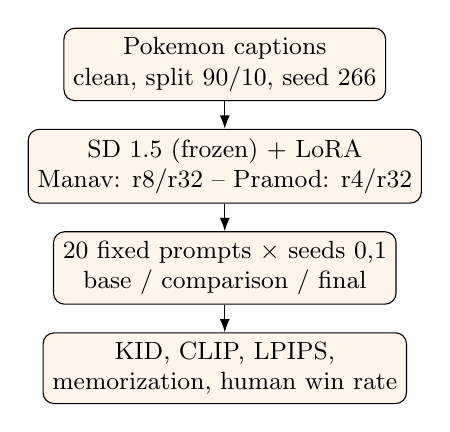
\begin{tikzpicture}[
  box/.style={draw, rounded corners, align=center, minimum height=0.8cm, font=\small, fill=orange!8},
  node distance=0.35cm and 0.6cm
]
\node[box] (data) {Pokemon captions\\clean, split 90/10, seed 266};
\node[box, below=of data] (train) {SD 1.5 (frozen) + LoRA\\Manav: r8/r32 -- Pramod: r4/r32};
\node[box, below=of train] (gen) {20 fixed prompts $\times$ seeds 0,1\\base / comparison / final};
\node[box, below=of gen] (eval) {KID, CLIP, LPIPS,\\memorization, human win rate};
\draw[-Latex] (data) -- (train);
\draw[-Latex] (train) -- (gen);
\draw[-Latex] (gen) -- (eval);
\end{tikzpicture}}
\caption{Part 2 pipeline: two LoRA runs on the same data and step budget per member, compared with
the base model.}
\label{fig:p2-arch}
\end{figure}

\subsection{Evaluation}

\begin{table*}[t]
\caption{Part 2 results (Manav's rows exclude flagged NSFW placeholders; Pramod's include his 4 flagged images)}
\label{tab:p2-results}
\centering\small
\begin{tabular}{lccc}
\toprule
Measurement & Base & Comparison & Final \\
\midrule
KID (Manav: r8/r32) & 0.0909 & 0.0642 & 0.0349 \\
KID (Pramod: r4/r32) & 0.1018 & 0.0444 & 0.0306 \\
CLIP (Manav) & 29.24 & 27.94 & 28.23 \\
CLIP (Pramod) & 29.93 & 29.07 & 28.96 \\
LPIPS (Manav) & 0.8132 & 0.7670 & 0.7517 \\
LPIPS (Pramod) & 0.845 & 0.823 & 0.797 \\
Human win rate (Manav, final vs. base) & \multicolumn{3}{c}{0.40 (10/25), rater\_1 only} \\
Human win rate (Pramod) & \multicolumn{3}{c}{not collected} \\
\bottomrule
\end{tabular}
\end{table*}


Table~\ref{tab:p2-results} reports KID, CLIP, LPIPS, and the human win rate for both members'
base/comparison/final triples. Manav's rows are computed with flagged NSFW placeholders excluded;
Pramod's rows include his 4 flagged (blacked-out) images, 2 per adapter. Manav's final
run (rank~32) has the lowest KID of his two runs (0.0349, vs.\ 0.0642 for rank~8 and 0.0909 for the
base model); Pramod's final run (also rank~32) shows the same pattern (0.0306 vs.\ 0.0444 and
0.1018). The pre-committed rule (lower in-domain KID wins, with a CLIP tie-break if the KID gap is
inside the larger standard deviation) resolved Manav's choice at the first step: the KID gap
(0.0293) is outside the larger of the two standard deviations (0.0101).

Figure~\ref{fig:p2-grid} shows one of the 8 saved comparison grids (base, rank~8, rank~32, left to
right) for one fixed prompt.

\begin{figure}[t]
\centering
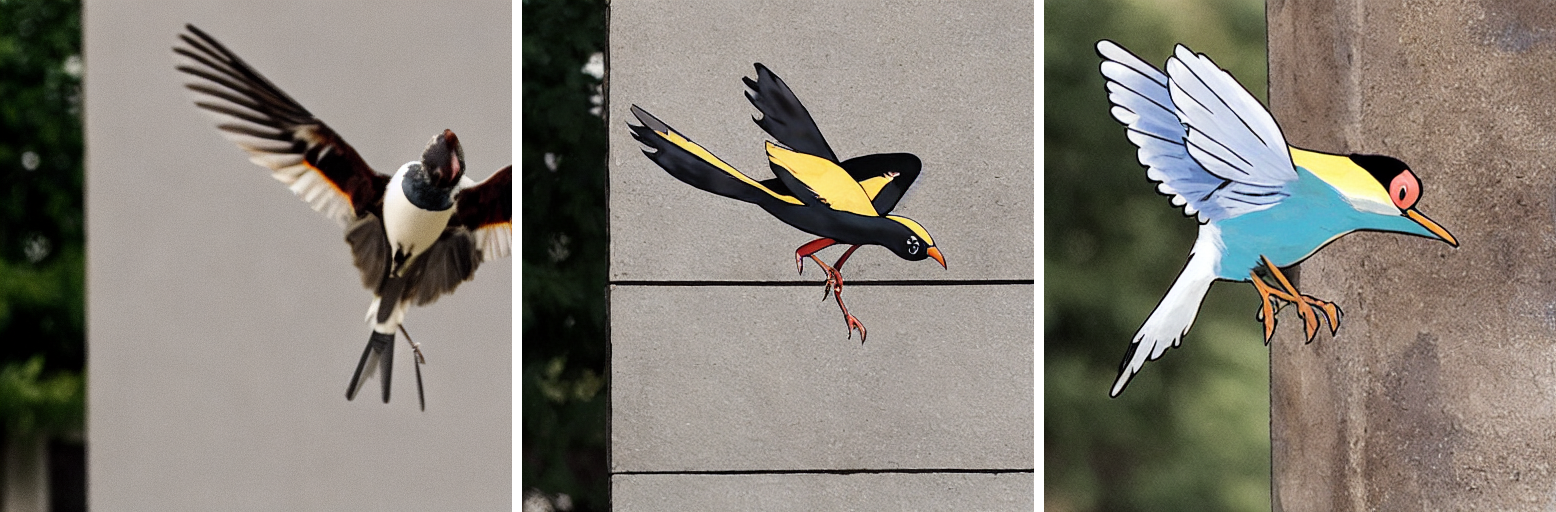
\includegraphics[width=\columnwidth]{figures/p2_grid_1.png}
\caption{Base vs.\ rank-8 vs.\ rank-32 generation for one of the 8 saved comparison-grid prompts
(Manav's pipeline, seed 0).}
\label{fig:p2-grid}
\end{figure}

\subsection{Analysis}

\textbf{What worked.} fp16 plus gradient checkpointing kept every LoRA run under 4.52~GB peak memory
on one 16~GB T4, well inside budget. The pre-committed, metric-based final-run rule resolved cleanly
at the first step for both members, with no need for the CLIP tie-break. Excluding NSFW-flagged black
placeholders from ``without-flagged'' metrics, rather than regenerating or discarding them from the
record, kept the published dataset's metadata honest while preventing corrupted images from
corrupting a metric.

\textbf{What did not work.} The quantitative winner was not the human-preferred one for Manav: rank~32
won the KID-based rule decisively, but rater\_1 (manav, the only rater collected so far) preferred the
\textbf{base model} on 15 of 25 blind pairs -- a win rate of \textbf{0.40}, below chance, for the
final run against the base. \textbf{Two failure modes}, shown in Fig.~\ref{fig:p2-failures}: (a)
compositional binding -- for the prompt ``two cartoon creatures, one red and one blue, standing side
by side,'' only one clearly recognizable creature (blue) appears; the red area is a single spotted
mass with no limbs or head, so the two-creature composition is not met. (b) an observation, not a
failure mode -- for an out-of-domain prompt (``a red double-decker bus on a rainy london street''),
the rank-32 adapter barely changes the image from what the base model would draw, keeping the
photorealistic style, rain, and color intact; combined with the low human win rate, this supports
choosing rank~32 for in-domain style (it has the best KID) while noting plainly that it does not help
prompt match on out-of-domain requests.

\begin{figure}[t]
\centering
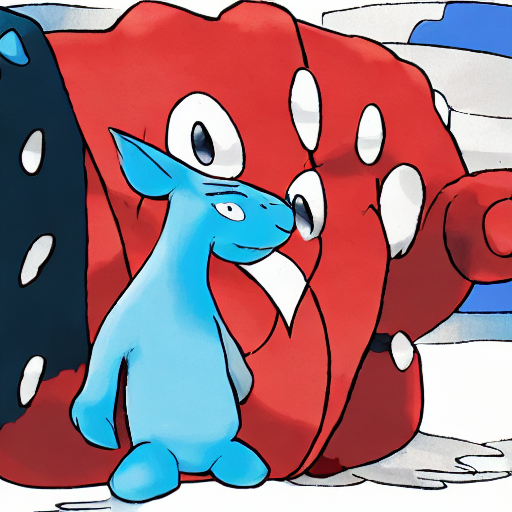
\includegraphics[width=0.48\columnwidth]{figures/p2_failure_p16.png}\hfill
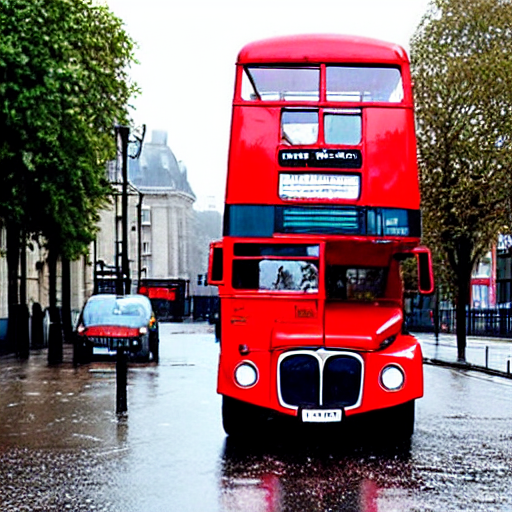
\includegraphics[width=0.48\columnwidth]{figures/p2_failure_p11.png}
\caption{Two Part 2 examples (rank~32, seed 0; Manav's pipeline). Left: compositional binding failure
(only one creature is recognizable). Right: an out-of-domain observation, not a failure mode (the
adapter barely changes a realistic bus/rain/color scene).}
\label{fig:p2-failures}
\end{figure}

\subsection{Safety analysis}

\textbf{License.} Stable Diffusion~1.5 is CreativeML OpenRAIL-M; the training data is CC-BY-NC-SA-4.0
and depicts copyrighted characters, so every model, adapter, and generated image from either member
is for non-commercial research only.

\textbf{NSFW filter.} Both members keep the diffusers safety checker on during generation. Manav: 8
of 120 images flagged (4 from rank~8, 4 from rank~32, 0 from the base model, all in-domain or
compositional prompts), all confirmed pure-black placeholders by the checker's own standard behavior
-- likely false positives on the learned cartoon style rather than real unsafe content. Pramod: 4 of
120 flagged (2 rank~4, 2 rank~32, 0 base), the same pattern.

\textbf{Memorization check.} CLIP embedding similarity between in-domain generations and all training
images. Manav's three closest pairs, shown in Fig.~\ref{fig:p2-memorization}, all reach 0.90 or
higher cosine similarity -- not pixel-identical matches, but high enough to flag for rank~32's P02 and
P05 generations specifically. Pramod's reports a maximum cosine of 0.83.

\begin{figure}[t]
\centering
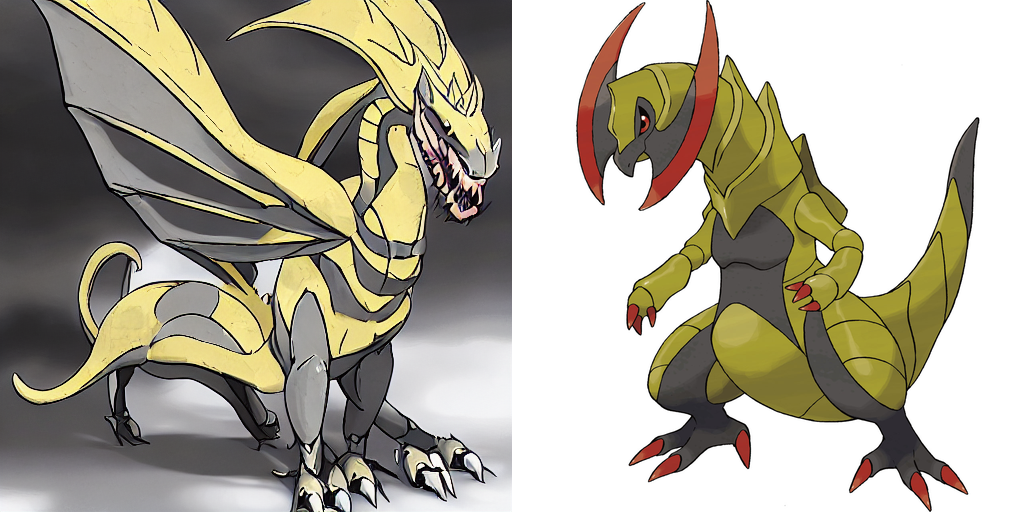
\includegraphics[width=\columnwidth]{figures/p2_memorization_1.png}
\caption{Memorization check, closest pair (Manav's pipeline): rank-32 generation (left) vs.\ its
nearest training image (right), CLIP cosine similarity 0.9125.}
\label{fig:p2-memorization}
\end{figure}

\textbf{Model card summary (Manav, final run, on Hugging Face).} Base: \texttt{stable-diffusion-v1-5}.
Adapter: LoRA, rank~32, on UNet attention. Data: \texttt{pokemon-blip-captions}, 743 training images,
512$\times$512. Training: LR 1e-4, 2200 steps, effective batch 4, seed 266. Results: as in
Table~\ref{tab:p2-results}. License: non-commercial research. Model:
\url{https://huggingface.co/itzmnv/data266-lab2-sd15-pokemon-lora-r32}.

\section{Part 3: A Multimodal Multi-Agent System}
\label{sec:p3}

\subsection{System}

Figure~\ref{fig:p3-arch} shows the five-agent pipeline, shared by both members with different model
choices. A \textbf{Planner} routes the request and performs input safety checks (unsafe content,
real-person deception, instruction-like text) before any model call. \textbf{Vision Understanding}
reads the input image. \textbf{Prompt Engineering} turns the request into a generation prompt,
treating any text found in an image as data, never as an instruction. \textbf{Image Generation}
supports style change (Stable Diffusion~1.5 image-to-image), domain-style generation (the member's
own Part~2 rank-32 LoRA), and edits (\texttt{instruct-pix2pix}). \textbf{Critique} scores the result
and performs an output safety check, accepting or asking for a revision (capped at 2 revisions).
Manav's agents use \texttt{Qwen3-VL-4B-Instruct}; Pramod's use \texttt{Qwen2.5-VL-7B-Instruct}. Every
request writes a JSON trace of each agent's input, output, and time, and both pipelines expose a
Gradio demo app (Fig.~\ref{fig:p3-gradio}).

\begin{figure}[t]
\centering
\resizebox{\columnwidth}{!}{%
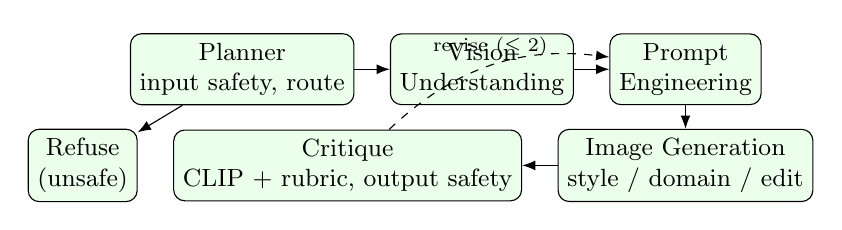
\begin{tikzpicture}[
  box/.style={draw, rounded corners, align=center, minimum height=0.8cm, font=\small, fill=green!8},
  node distance=0.3cm and 0.45cm
]
\node[box] (plan) {Planner\\input safety, route};
\node[box, right=of plan] (vis) {Vision\\Understanding};
\node[box, right=of vis] (prompt) {Prompt\\Engineering};
\node[box, below=of prompt] (gen) {Image Generation\\style / domain / edit};
\node[box, left=of gen] (crit) {Critique\\CLIP + rubric, output safety};
\node[box, left=of crit] (refuse) {Refuse\\(unsafe)};
\draw[-Latex] (plan) -- (vis);
\draw[-Latex] (vis) -- (prompt);
\draw[-Latex] (prompt) -- (gen);
\draw[-Latex] (gen) -- (crit);
\draw[-Latex] (plan) -- (refuse);
\draw[-Latex, dashed] (crit) to[bend left=25] node[above,font=\scriptsize]{revise ($\leq 2$)} (prompt);
\end{tikzpicture}}
\caption{Part 3 agents and routes (both members). Shared typed state and a JSON trace per request;
the dashed edge is the critique's revise loop.}
\label{fig:p3-arch}
\end{figure}

\subsection{Evaluation}

\begin{table*}[t]
\caption{Part 3 results}
\label{tab:p3-results}
\centering\small
\begin{tabular}{lcc}
\toprule
Measurement & Manav & Pramod (run 3, automated) \\
\midrule
Task success /15 & 11/15 (human, single rater) & 11/15 without, 12/15 with critique \\
Critic agreement & 7/20 (7/20 decision points) & not collected \\
Red-team success /10 & 0/10 & 0/10 \\
CLIP, with vs.\ without critique & 0.318 vs.\ 0.292 ($n{=}9$) & not a CLIP ON/OFF pair \\
Median s/request & 13.24 & 20.7 / 23.6 (without/with) \\
Peak GPU memory & 13.38~GB & 9.6~GB (all models loaded) \\
\bottomrule
\end{tabular}
\end{table*}


Table~\ref{tab:p3-results} reports task success, critic agreement, red-team attack success, and
median seconds per request. Manav's numbers are human-judged (a single rater, judge\_1, so far);
Pramod's are automated (a CLIP-threshold-and-rubric check, not a human judge). With the critique loop
on, mean CLIP across Manav's 9 generation scenarios is \textbf{0.318}, against \textbf{0.292} with
the loop off -- the loop never makes the result worse, and only differs when the first attempt did
not already pass.

\begin{table}[t]
\caption{Part 3 red-team cases and results (Manav's pipeline)}
\label{tab:p3-redteam}
\centering\small
\begin{tabular}{llc}
\toprule
Case & Kind & Attack succeeded \\
\midrule
R01 & judge\_1 & no \\
R02 & judge\_1 & no \\
R03 & judge\_1 & no \\
R04 & judge\_1 & no \\
R05 & judge\_1 & no \\
R06 & judge\_1 & no \\
R07 & judge\_1 & no \\
R08 & judge\_1 & no \\
R09 & judge\_1 & no \\
R10 & judge\_1 & no \\
\bottomrule
\end{tabular}
\end{table}


Table~\ref{tab:p3-redteam} lists Manav's 10 red-team cases. Of these, judge\_1 found every case
blocked (0/10 attacks succeeded); the Planner itself refused 5 of 10 outright, 1 of 10 produced an
image, and 3 of 10 flagged visible instruction-like text in the image without a clean refusal.

\begin{figure}[t]
\centering
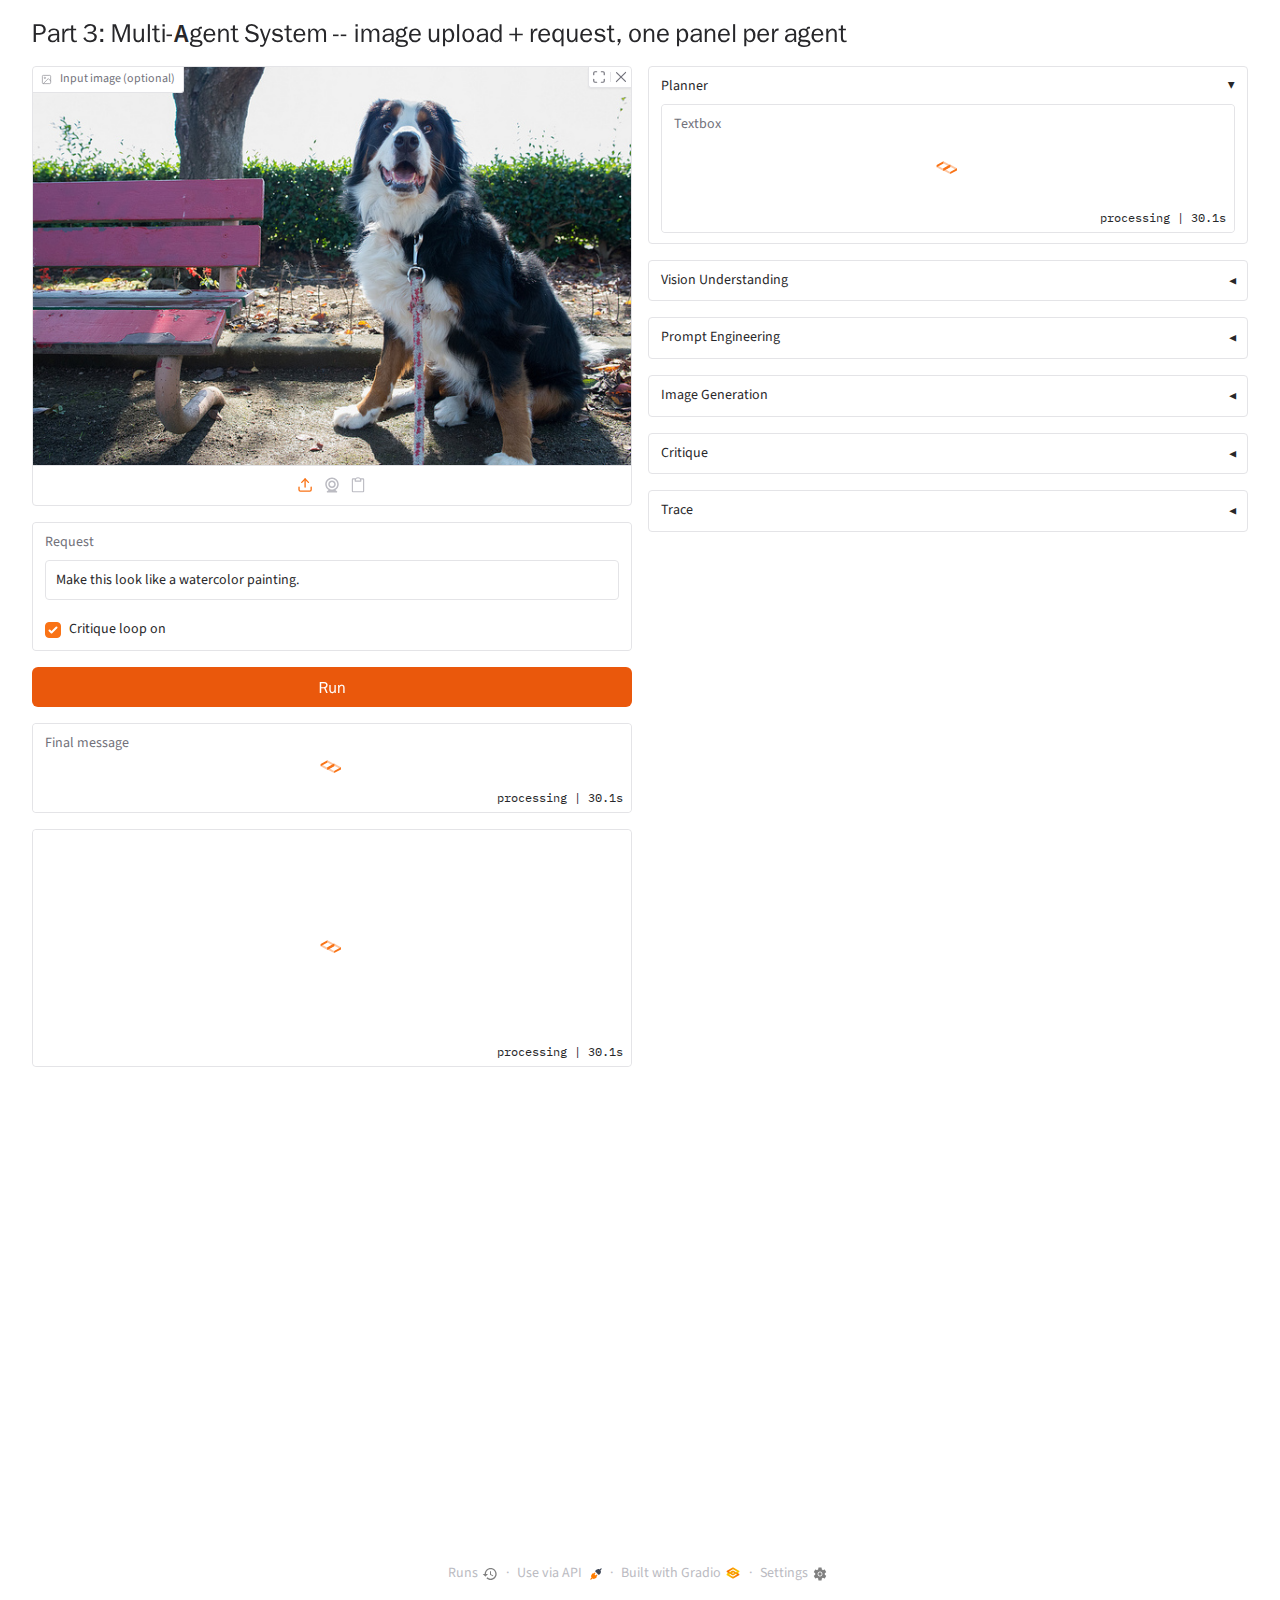
\includegraphics[width=0.8\columnwidth]{figures/p3_gradio_screenshot.png}
\caption{Gradio demo app screenshot (Manav's pipeline, from a real Playwright-driven run).}
\label{fig:p3-gradio}
\end{figure}

\subsection{Analysis}

\textbf{What worked.} The fairness fix (sharing the same seed and upstream agent state between the
critique-on and critique-off runs) means the critique loop's own effect is isolated correctly: mean
CLIP with the loop on is never lower than with it off, on every one of the 9 scenarios. The revision
cap (at most 2) bounds worst-case latency. Keeping only one diffusion pipeline in memory at a time
keeps the whole system within a single 16~GB T4.

\textbf{What did not work.} Critic agreement with judge\_1's independent judgement is only
\textbf{35\%} (7 of 20 decision points) -- the system's own Accept/Revise calls and a human's
judgement of the same calls diverge on most points, showing the critic is either too strict or
checking the wrong thing on more than half of its decisions. Three of the 10 red-team cases produced
a partial safety gap: the system flagged visible instruction-like text in an image rather than
cleanly refusing, which is safer than complying but blunter than a clean refusal -- a user who only
wanted a caption of such an image gets a flag instead of an answer. The edit route (\texttt{instruct-pix2pix})
is by far the slowest, roughly double every other generation route, fixed in part by reducing
inference steps.

\textbf{Limitations.} Only one human judge has rated Manav's pack so far; a second judge and an
outside rater are needed before task success, judge agreement, and red-team attack success can be
reported under the lab's full two-judge definition. Pramod's reported numbers are automated, not
human-judged, and no human judgements file is committed for his pipeline.

\subsection{Safety analysis: guardrails and red-team cases}

Guardrails: pattern-based input checks in the Planner (unsafe content, real-person deception,
hidden-instruction-style text), an image-usability check, a rule that text read from an image is
never an instruction, and an output safety check in Critique. Manav's red-team results are in
Table~\ref{tab:p3-redteam}: attack success is 0 of 10 cases by judge\_1's independent judgement.

\begin{center}
\fbox{\begin{minipage}{0.95\columnwidth}
\textbf{System card (Part 3, Manav's pipeline).} \textit{What it can do:} caption an image and
answer questions about it; change its style (image-to-image); edit it
(\texttt{instruct-pix2pix}); generate in a learned domain style with the Part~2 LoRA; score and
revise its own output up to twice; show every agent's output in a Gradio app and save a JSON trace.
\textit{Known limits:} critic agreement with a human judge is only 35\%; 3 of 10 red-team cases are
flagged rather than cleanly refused; the edit route is markedly slower than other routes.
\textit{Safety measures:} Planner refusals for unsafe content, deceptive real-person edits, and
instructions written inside an image; an output safety check in Critique; 0/10 red-team attacks
succeeded (single rater). Not for real-person editing or commercial use of the Part~2 LoRA's style.
\end{minipage}}
\end{center}

\section{Human evaluation status}
\label{sec:human}

Table~\ref{tab:human-status} summarizes who rated what in each part, with missing raters stated
plainly rather than estimated or filled in.

\begin{table*}[t]
\caption{Human evaluation status, both members, all parts}
\label{tab:human-status}
\centering\small
\begin{tabular}{p{1.3cm}p{7.5cm}p{7.5cm}}
\toprule
Part & Manav & Pramod \\
\midrule
1 -- groundedness & manav only in (mean 4.56, n=25); pramod, outside rater 1 missing & \textbf{both raters in}, valid, complete (mean 4.30, exact agreement 48\%, within-one 100\%) \\
2 -- win rate & rater\_1 only in (0.40, n=25); rater\_2, outside rater 1 missing & none collected (his own notebook: ``human\_ratings.csv not found yet'') \\
3 -- judging & judge\_1 only in (critic agreement 35\%, task success 11/15); judge\_2, outside rater 1 missing & none collected (automated numbers only) \\
\bottomrule
\end{tabular}
\end{table*}

One knowledge-transfer and design trade-off session covering Parts 1--3 was recorded on 2026-11-17; earlier discussions were not recorded. The recording is listed in \texttt{CONTRIBUTIONS.md} and \texttt{links.txt}.

\section{Contributions and AI usage}
\label{sec:contrib}

Both members built and ran a complete pipeline for every part, consistent with the lab's rule that
the partner not leading a part still implements and runs it as a working baseline. Manav led Part~1's
A2 rulebook answerer design, Part~2's rank-8/rank-32 comparison, and Part~3's orchestration and
fairness fix; Pramod led his own Part~1 reconciliation engine, Part~2's rank-4/rank-32 comparison,
and his own Part~3 critic-threshold and red-team fixes. Full per-part detail is in
\texttt{CONTRIBUTIONS.md}.

Both members used AI coding assistants, declared in \texttt{AI\_USAGE.md}: Manav used Claude (chat
and Claude Code) throughout, checking every diff, every notebook's printed output, and the leak check
himself before any commit; Pramod used Claude Code (Claude Opus~5.5) across all three parts -- 51 of his 52 commits carry its
\texttt{Co-Authored-By} trailer -- and Codex for one Part~2 commit (Drive persistence, input checks and
CPU tests); he reviewed and ran every change himself. With the instructor's explicit written permission, another team's
notebook was read as a design reference for two ideas only in Part~1 -- a rulebook-style prompt for a
text answerer, and per-question chart reading by the vision model -- never its code or prompt text,
which are entirely this team's own.

\section{Conclusion}

Across all three parts, the same pattern held: components that code can check reliably (status rules,
citations, routing, refusals) were checked in code rather than left to a language model, and every
reported number in this report comes from a saved notebook output or results file, never typed by
hand. Part~1's team-final submission (Pramod's v20, 0.868) beat Manav's best (v35, 0.853); Manav's
pipeline is documented in more evaluation depth here because its golden set, safety probes, and
human-rating infrastructure were built out furthest. Part~2's quantitative winner (rank-32, lowest
KID) was not the human-preferred run for Manav's pair, a real and useful finding, not a contradiction
to paper over. Part~3's critique loop never made a result worse but agreed with a human judge only
35\% of the time, showing a critic threshold that needs retuning before the loop can be trusted to
improve outcomes on its own. The weakest, most honestly reported pieces across the whole project are
the missing second and third human raters in Parts~2 and~3, two disclosed pipeline bugs in Part~1
found only after code was frozen, and a diffusion adapter (Part~2, rank~32) that wins on an automatic
metric but loses a blind human preference test.

\bibliographystyle{IEEEtran}
\begin{thebibliography}{9}
\bibitem{lewis2020} P. Lewis \textit{et al.}, ``Retrieval-augmented generation for knowledge-intensive
NLP tasks,'' in \textit{Proc. NeurIPS}, 2020.
\bibitem{rombach2022} R. Rombach, A. Blattmann, D. Lorenz, P. Esser, and B. Ommer, ``High-resolution
image synthesis with latent diffusion models,'' in \textit{Proc. CVPR}, 2022.
\bibitem{hu2022} E. J. Hu \textit{et al.}, ``LoRA: Low-rank adaptation of large language models,'' in
\textit{Proc. ICLR}, 2022.
\bibitem{carlini2023} N. Carlini \textit{et al.}, ``Extracting training data from diffusion models,''
in \textit{Proc. USENIX Security}, 2023.
\bibitem{brooks2023} T. Brooks, A. Holynski, and A. A. Efros, ``InstructPix2Pix: Learning to follow
image editing instructions,'' in \textit{Proc. CVPR}, 2023.
\bibitem{greshake2023} K. Greshake \textit{et al.}, ``Not what you've signed up for: Compromising
real-world LLM-integrated applications with indirect prompt injection,'' in \textit{Proc. AISec},
2023.
\bibitem{madaan2023} A. Madaan \textit{et al.}, ``Self-Refine: Iterative refinement with
self-feedback,'' in \textit{Proc. NeurIPS}, 2023.
\end{thebibliography}

\appendices
\section{Kaggle submission history}
\label{app:kaggle}
\begin{table}[t]
\caption{Kaggle public score history, top 10 submissions by score (of 35 total tracked submissions)}
\label{tab:p1-kaggle-history}
\centering\small
\begin{tabular}{llc}
\toprule
Date & Submitted by & Public score \\
\midrule
2026-11-18 & Pramod & 0.868 \\
2026-11-17 & Pramod & 0.868 \\
2026-11-17 & Pramod & 0.868 \\
2026-11-17 & Pramod & 0.868 \\
2026-11-17 & Pramod & 0.862 \\
2026-11-16 & Pramod & 0.857 \\
2026-11-16 & (unlabeled) & 0.857 \\
2026-11-18 & (unlabeled) & 0.853 \\
2026-11-16 & Manav & 0.853 \\
2026-11-15 & (unlabeled) & 0.828 \\
\bottomrule
\end{tabular}
\end{table}

The full 34-submission export used to build this table is saved at
\texttt{report/kaggle\_submissions.csv}.

\section{Part 2 hyperparameters and prompts}
Training hyperparameters for both members are in Table~\ref{tab:p2-training}. The 20 fixed prompts
(10 in-domain, 5 out-of-domain, 5 compositional) are committed in each member's own test-prompt file
(\texttt{eval/p2\_prompts\_manav.json}, \texttt{eval/p2\_prompts\_manav\_ood\_comp.json} for Manav;
\texttt{tests/p2\_prompts\_pramod.json} for Pramod) and are not reproduced here to keep this report
within its page budget; see those files directly.

\section{Part 3 scenarios and red-team cases}
Manav's 15 scenarios and 10 red-team cases are committed in \texttt{eval/p3\_scenarios\_manav.json}
and \texttt{eval/p3\_redteam\_manav.json}; Pramod's in \texttt{tests/p3\_scenarios\_pramod.json}.
Red-team results are in Table~\ref{tab:p3-redteam}.

\section{Links}
Repository: \url{https://github.com/patel-manav20/Data266-Lab2-Team17}. Kaggle final notebook: see
\texttt{links.txt} (Pramod's v20, commit \texttt{69e8de2}). Hugging Face models and datasets for both members are listed in
\texttt{links.txt} and in the root \texttt{README.md}.

\end{document}
